\documentclass[11pt, titlepage]{article}
\usepackage[a4paper, total={150mm, 260mm}]{geometry}
\usepackage[utf8]{inputenc}
\usepackage{subfigure}
\usepackage{float}
\usepackage{graphicx}
\graphicspath{ {images/} }
\usepackage{xcolor}
\usepackage{hyperref}
\hypersetup{
	colorlinks,
	linkcolor={red!50!black},
	urlcolor={blue!80!black}
}
\title{Tom's Git Guide}
\author{Tom Schwarz\thanks{with contributions from Ben Schwarz}}
\date{Janurary 2019\\v1.A} %letters for pre-releases, .0 for main release, .1+ for post-updates

\begin{document}
\maketitle

\tableofcontents

\section{Introduction}
This guide was written to explain how to use git (and GitHub) quickly and easily. While it definitely is not a particularly good guide, I couldn't find one online that explained, practically, how to use git with the right context and simply enough. So I wrote this. For an explanation of how Git works (which you \emph{must} know before you read this (knowing ``git commit'', ``git pull'' and ``git push'' or their equivalent GUI buttons dosen't count)) see \href{https://blog.red-badger.com/2016/11/29/gitgithub-in-plain-english}{Git \& Github in plain english} (seriously - do read it).

\pagebreak

\section{Solving merge conflicts (in VS Code)}
\label{sec:solving_merge_conflicts}
Merge conflicts occur when git is trying to merge converged histories, and in the process finds both groups have edited the same file. For example, this can occur when:
\begin{itemize}
	\item You run ``git pull'' after you have commited changes to a file, and someone else has commited and pushed different changes to the same file
	\item You merge a branch back to master, after you changed a file in the branch and someone else changed the same file in master
	\item You are updating your branch to have new changes from master - ie the reverse of above
\end{itemize}
Luckily solving merge conflicts is much less spooky than it appears:
\begin{enumerate}
	\item Firstly you will be notified that a merge conflict has occured either by some sort of error message after running ``''git merge conflicting-branch'' that looks like ``CONFLICT (content): Merge conflict in file.txt / Automatic merge failed; fix conflicts and then commit the result.'' or the following error dialog box if using the GUI:
	\begin{figure}[H]
		\centering
		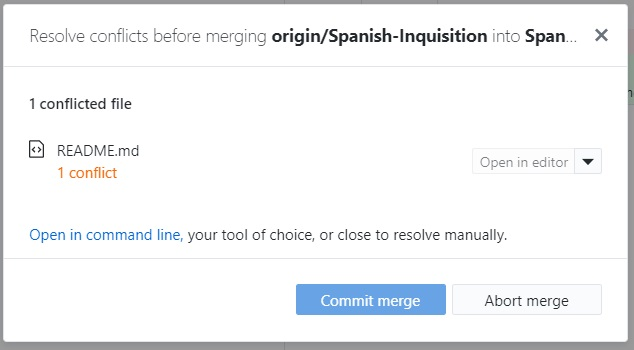
\includegraphics[width=0.5\textwidth]{SMC/1conflict-dialog}
		\caption{The horror! The horror!}
	\end{figure}
	\item To solve the conflict, simply open the conflicting file(s) in your favourite text editor, and make the file look exactly how you want it. In this case we will use Visual Studio Code, but any text editor works:
	\begin{figure}[H]
		\centering
		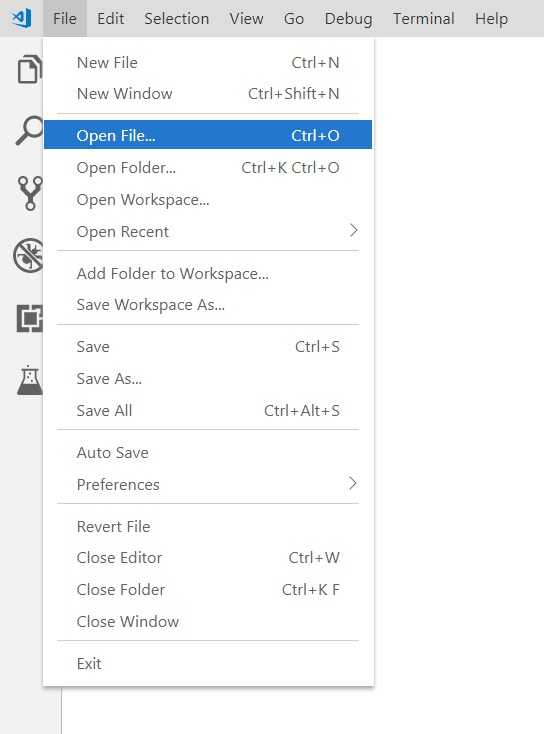
\includegraphics[width=0.5\textwidth]{SMC/2open-file}
		\caption{Open the file in VS Code by going File \textgreater Open File... and selecting it. It can be any type of (text) file - not necessarily just .java or whatever you commonly edit in VS Code.}
	\end{figure}
	The general structure of the file will be:
	\begin{table}[H]
		\begin{tabular}{p{0.35\linewidth} p{0.65\linewidth}}
		Preceding context code & \\
		 $<<<<<<<$ HEAD & This indicates the start of the conflicting section, and that this first section corresponds to the HEAD commit - ie your commit. VS Code has helpfully labelled this as the (Current Change). \\
		  Blah Blah text &  \\
		 =======& This indicates the dividor between your code, and the alternative commit code \\
		 Blah Blah conflicting text&  \\
		 $>>>>>>>$ 123456& This indicates the end of the conflicting section, and gives the reference hash for the alternative commit code. VS Code has helpfully labelled this as the (Incoming Change) \\
		 Ending context code & 
		\end{tabular}
	\end{table}
	Here is an example file:
	\begin{figure}[H]
		\centering
		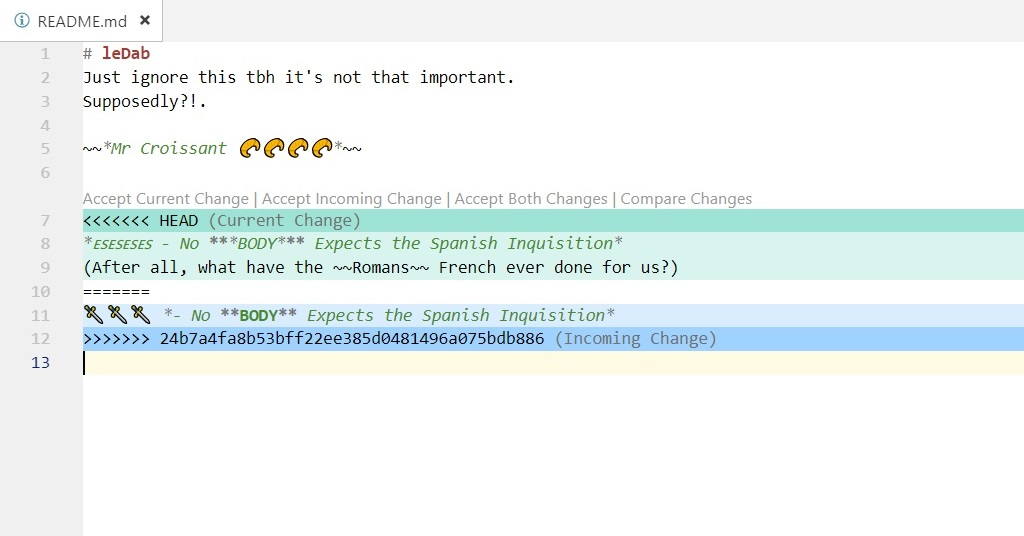
\includegraphics[width=\textwidth]{SMC/3conflicted-file}
		\caption{The opened file. VS Code has added the colouring and light grey help text}
	\end{figure}
	\item Now edit the file to look how you want. You can use VS Code's handy buttons to choose the current change or incoming change or both changes (or get a side-by-side diff). You can also just ignore it all together and touch up the file yourself. Generally I click ``Accept Both Changes'' to have it remove the \textless, = and \textgreater stuff and then fix up the code myself - but do what makes sense in the situation
	
	
Note: Often, merge conflicts are minor issues that you can just quicly touch up. However, if you don't communicate with other team members its possible that you can have an actual logical merge conflict -eg you both edited the same function to do something you want. In this case you will need to re-code the function, and the code that uses it, to solve the conflict (even though git might say its been solved before then, you still need to update the dependant code)
	\begin{figure}[H]
		\centering
		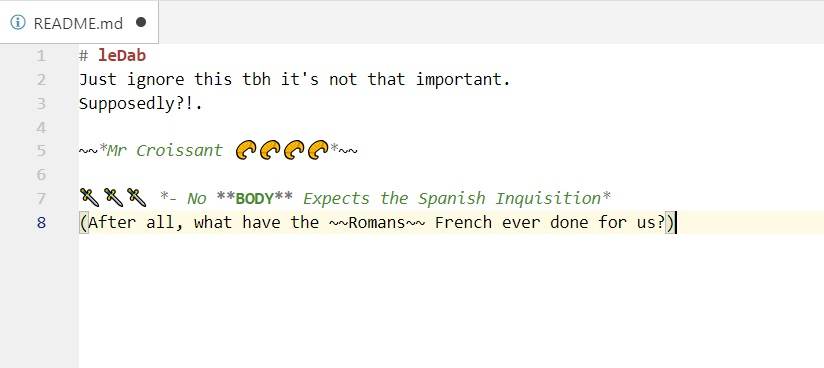
\includegraphics[width=\textwidth]{SMC/4merge-resolved}
		\caption{Note that the merge has been fully resolved, and the file looks exactly as we want it.}
	\end{figure}
	\item Save and test your code. (This is a very important, non-skippable step. Don't skip it.)
	\item Run ``git commit'' to finish the merge, or go back to the GUI and click ``commit merge'' (Alternatively you can run git merge --abort to stop merging, and return the branch to how it was before you tried to merge).
\end{enumerate}
For more help on solving merge conflicts, see this \href{https://www.atlassian.com/git/tutorials/using-branches/merge-conflicts}{Atlassian Git merge conflicts} article.


\section{Branching \& Pull Request Workflow}
\label{sec:branching_pull_request_workflow}
This explains a simple workflow, but in extreme detail. A quick outline of this workflow:
\begin{enumerate}
	\item Create a branch and work on your new changes there
	\item Create a pull request to incorporate changes into master
	\item Review \& approve the pull request, making changes as necessary
	\item Delete the branch
\end{enumerate}

\subsection{Creating a branch}
\label{sec:BPRW_creating_branch}
\begin{enumerate}
	\item Make sure your git repo is up to date with origin (ie Github) - either by running ``git pull'' or in the GUI clicking the ``Fetch origin'' button
	\item Create the branch by running ``git checkout -b your-branch-name'' or in the GUI going ``Branch \textgreater New Branch'' (also available from the ``current branch'' button next to fetch origin).
	\item Choose a suitable branch name, compliant with relevant conventions/guidelines - it should be short and descriptive. You should create a new branch for every self-contained feature - do NOT create large monolithic branches for miscellaneous updates; even if it means having a branch with just one commit.
	\item Add this branch to origin either by running ``git push --set-upstream origin your-branch-name'' (the extra option connects your new branch to a new reflected branch in origin) or hitting the ``Publish branch'' button in the GUI.
	\begin{figure}[H]
		\centering
		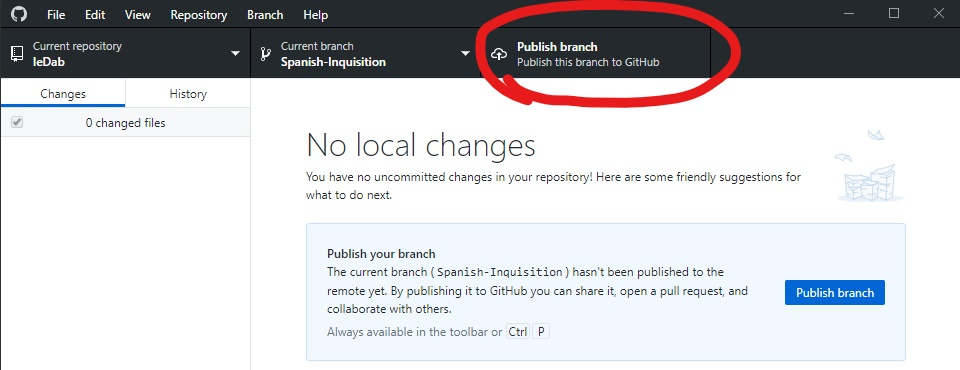
\includegraphics[width=\textwidth]{BPRW/1publish-branch}
		\caption{The publish branch button in the GUI}
	\end{figure}
	\item Now you can start working on your feature, updating code, making commits and pushing them up to Github as normal!
	\begin{figure}[H]
		\centering
		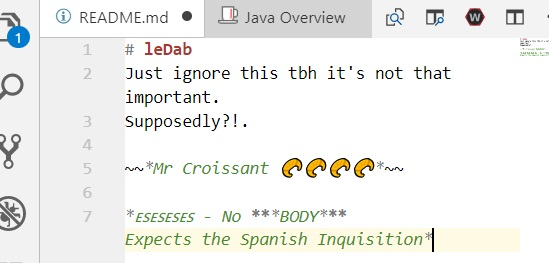
\includegraphics[width=0.75\textwidth]{BPRW/2modified-file}
		\caption{These important files have been modified (\&commited) in the branch}
	\end{figure}
\end{enumerate}

\subsection{Creating the pull request}
\label{BPRW_creating_pull_request}
\begin{enumerate}
	\item First, we must encorporate any changes that have been made to master while we have been working on our branch.
	\begin{enumerate}
		\item Update the local copy of master using ``git checkout master'' and ``git pull'' or in the GUI clicking the ``Fetch origin'' button
		\item Next, merge these changes into your branch by checking out your feature branch and running ``git merge master'' or in the GUI going ``Branch \textgreater Update from master''. You may need to resolve merge conflicts - if so, see the \hyperref[sec:solving_merge_conflicts]{Solving merge conflicts} section.
	\end{enumerate}
	\item sync your merge changes with origin (``git push'' or the sync button)
	\item Go to the github website for the repository, changing to your feature branch
	\begin{figure}[H]
		\centering
		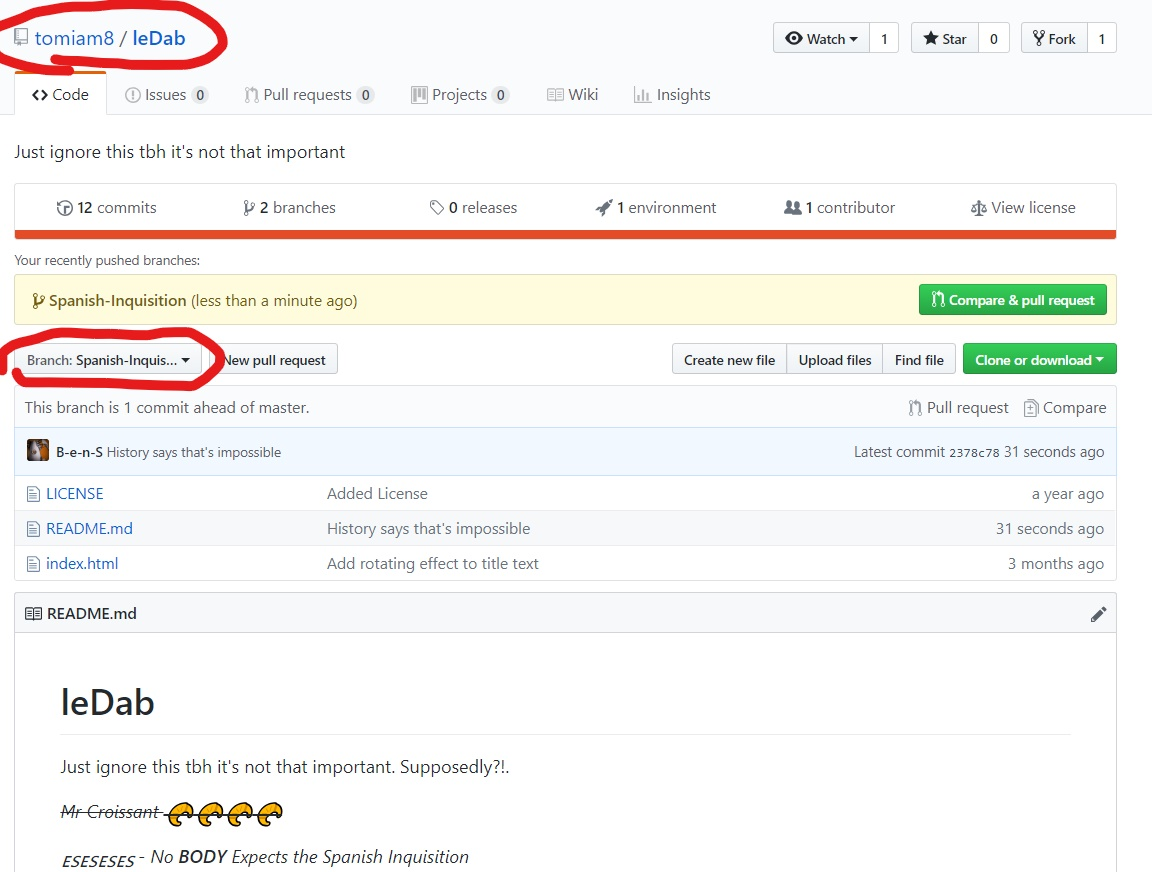
\includegraphics[width=0.8\textwidth]{BPRW/3github-website}
		\caption{Note that we have selected the repository, and the feature branch}
	\end{figure}
	\item Create the pull requst
	\begin{enumerate}
		\item Click on the ``pull request'' button
		\begin{figure}[H]
			\centering
			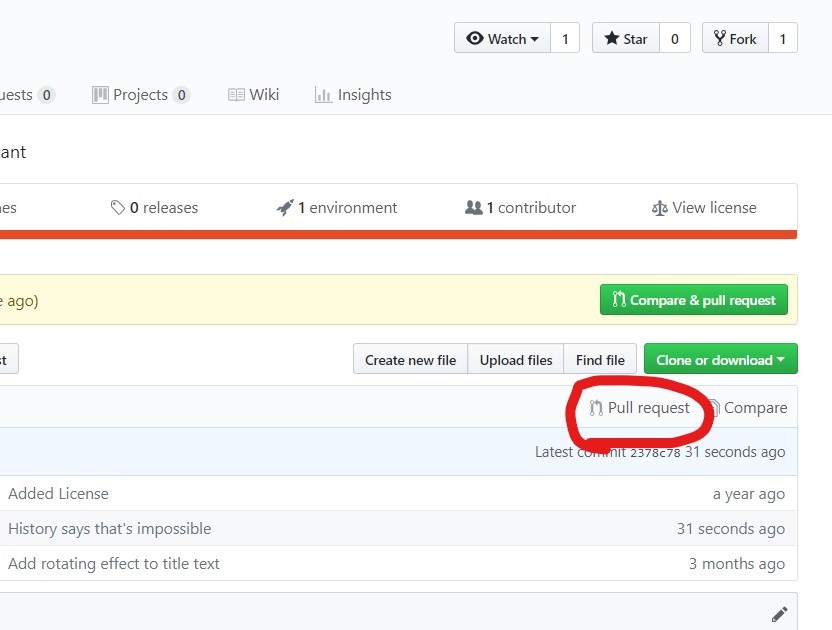
\includegraphics[width=0.8\textwidth]{BPRW/4start-pull-request}
			\caption{Click the ``pull request'' button to create the pull request}
		\end{figure}
		\item Check the branches are correct (master on left, feature branch on right)
		\item create a helpful title and comment
		\item Review the code changes shown below
		\item Create the pull request
		\begin{figure}[H]
			\centering
			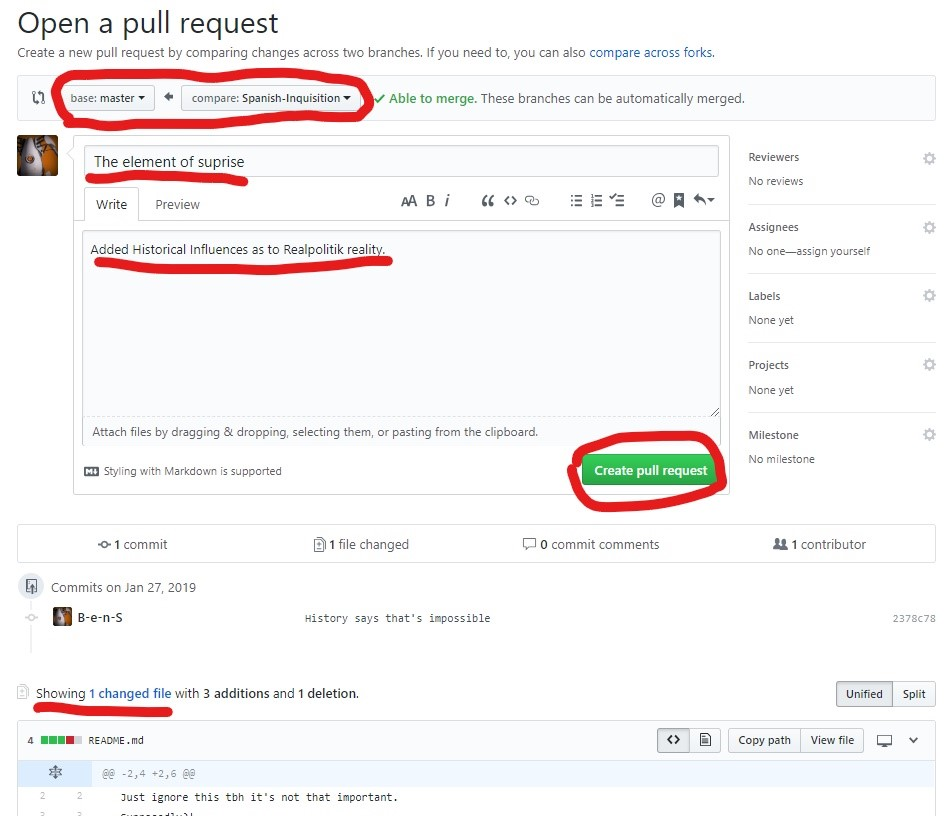
\includegraphics[width=\textwidth]{BPRW/5create-pull-request}
			\caption{Do the things}
		\end{figure}
	\end{enumerate}
	\item Now, just get a programming leader to review your pull request!
\end{enumerate}

\subsection{Reviewing the pull request}
\label{BPRW_reviewing_pull_request}
Note that this subsection is only intended for those reviewing the pull request (i.e. doing the code review) - but it can still be useful to read it anyway!
\begin{enumerate}
	\item Select, open and view the pull request by clicking ``Pull Requests'' (in the top bar, right below the repository name) \textgreater The pull request name:
	\begin{figure}[H]
		\centering
		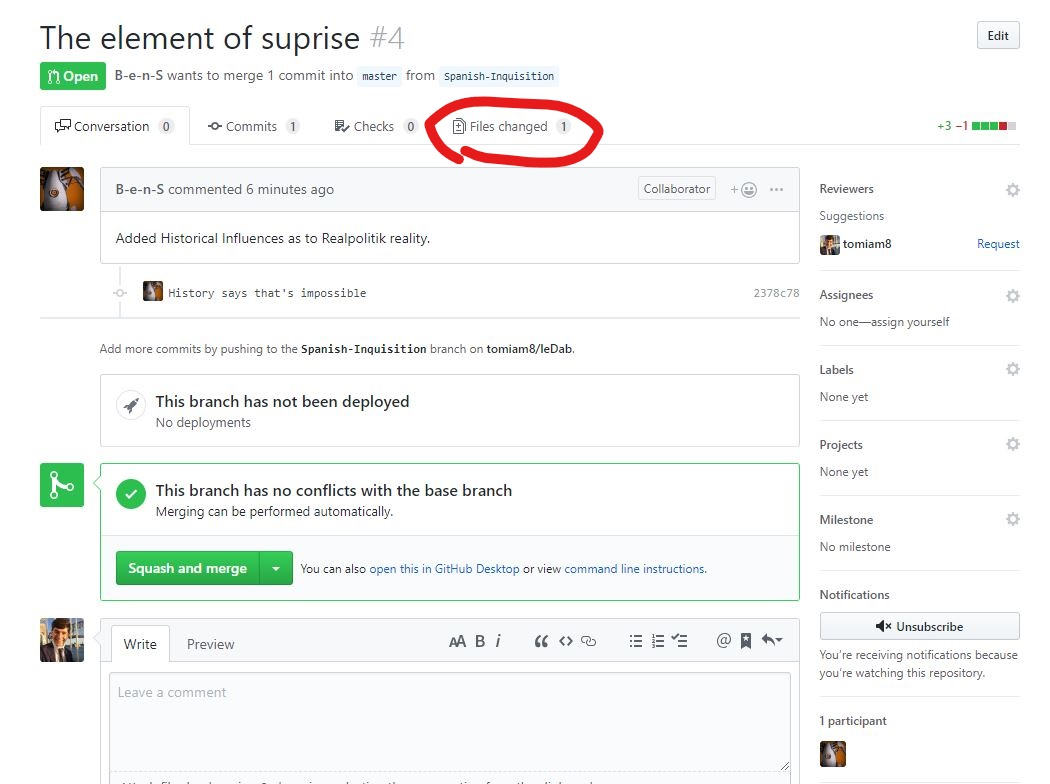
\includegraphics[width=\textwidth]{BPRW/6view-pull-request}
		\caption{Yay do the things}
	\end{figure}
	\item Click ``Files changed'' to view the code updates in the pull request, and begin the review.
	\item Click individual lines (near the line numbers) to add comments to individual lines of the file, and click ``review changes'' to make a general comment. You can change the ``Diff settings'' to see more of the file. For individual line comments you can make code suggestions for very simple changes, that can be easily accepted by the pull request proposer. For the general comment you can just make a comment, accept the pull request, or request code changes. For this example, we'll be demonstrating asking for additonal changes.
	\begin{figure}[H]
		\centering
		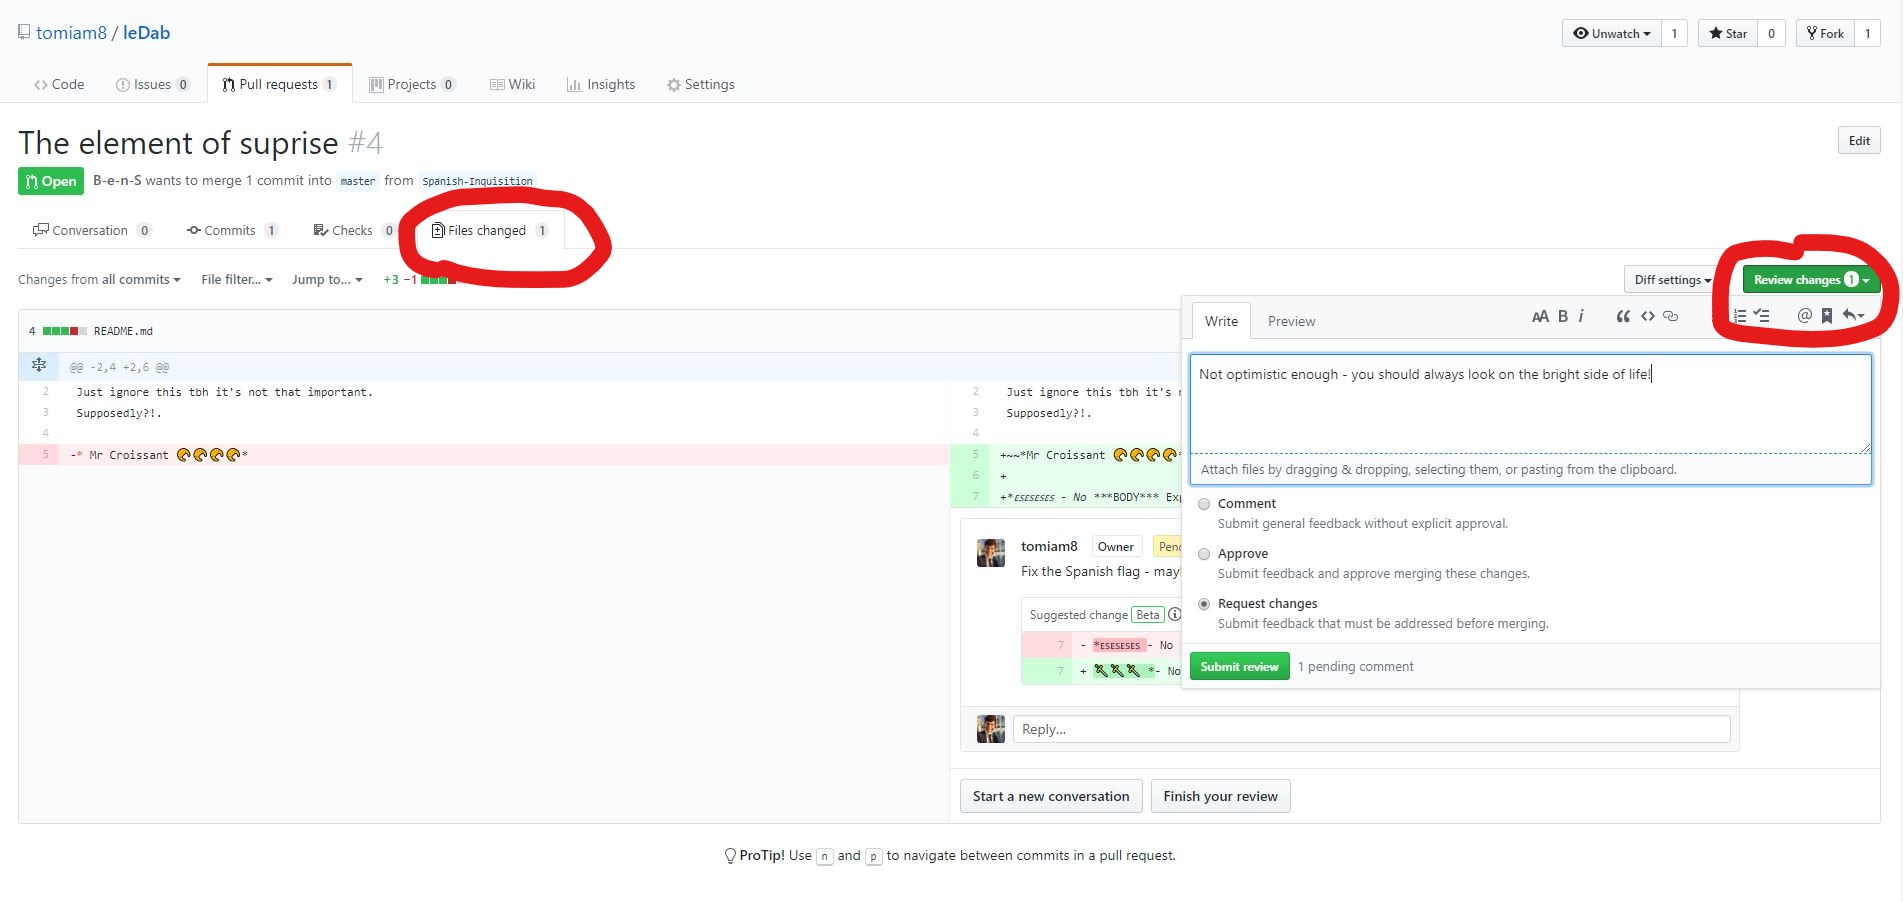
\includegraphics[width=\textwidth]{BPRW/7code-review}
		\caption{Note how the code has been reviewed}
	\end{figure}
\end{enumerate}

\subsubsection{Making changes}
\label{BPRW_RPW_making_changes}
This section details how to edit/update the pull request, eg after the code reviewer has requested changes
\begin{enumerate}
	\item Open the pull request and view the comment
	\begin{figure}[H]
		\centering
		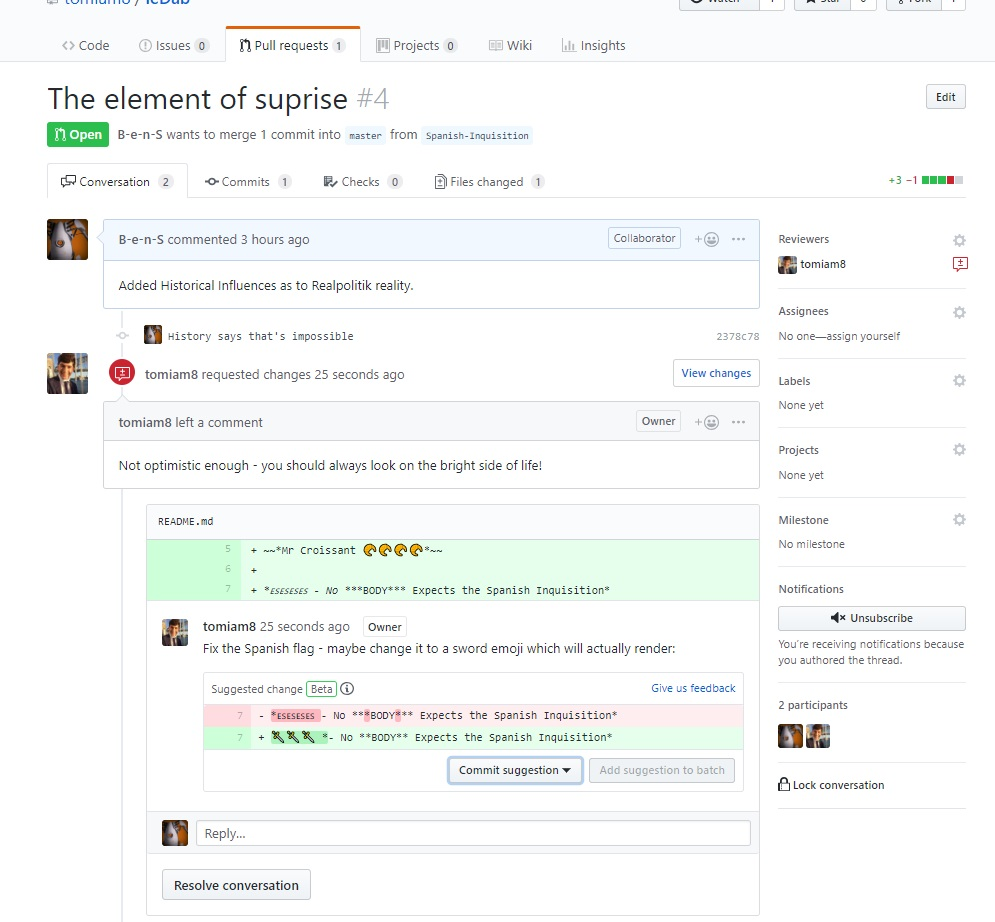
\includegraphics[width=\textwidth]{BPRW/8view-comment}
		\caption{Look at all these lovely comments. Also, note how you can commit the code suggestion instantly!(You will need to re-pull if you do this)}
	\end{figure}
	\item Simply create a new commit to the feature branch, and push it to github. Notify the code-reviewer that you have met their tyrannical demands.
\end{enumerate}

\subsubsection{Approving the pull request}
\label{BPRW_RPW_approving_pull_request}
Again this is for the code reviewer!
\begin{enumerate}
	\item Open up the code review on Github.com
	\item View the changes as before (or, you can view the individual commit to see what changed) and then approve the changes, or create an additional request for changes as before.
	\begin{figure}[H]
		\centering
		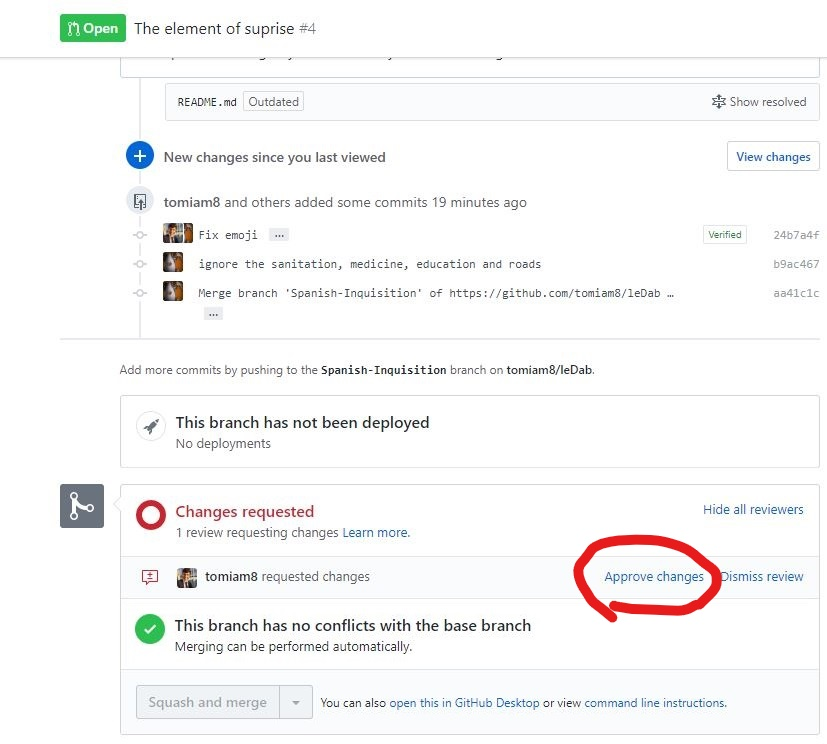
\includegraphics[width=\textwidth]{BPRW/9approve-changes}
		\caption{Click the approve changes button to approve the changes}
	\end{figure}
	\item Then click ``merge'' (the big green button) to merge the pull request. You can choose between creating a new ``merge'' commit, squashing the commits into a mega-commit or rebasing (append the commits to the end of master).
\end{enumerate}

\subsection{cleanup}
\label{BPRW_cleanup}
\begin{enumerate}
	\item As you can see, we have finished the merge and master has the new feature! Now however we must go ahead and delete the existing branch.
	\begin{figure}[H]
		\centering
		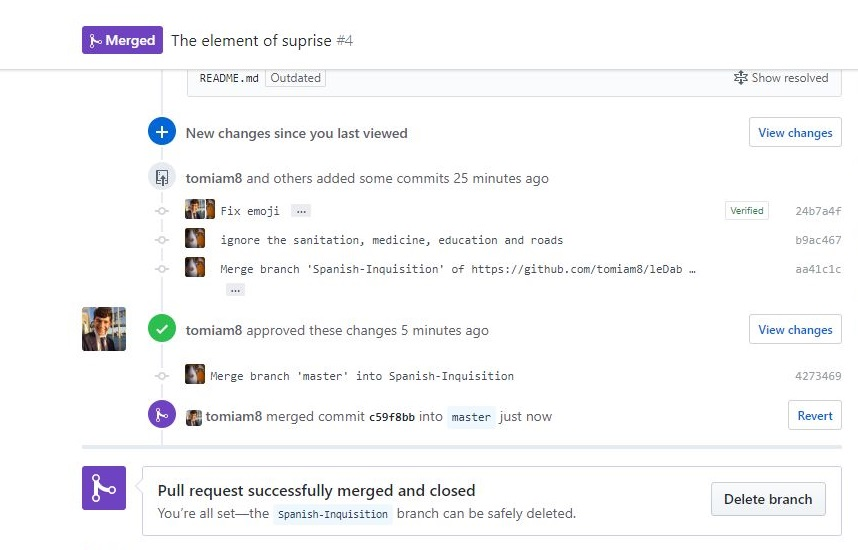
\includegraphics[width=\textwidth]{BPRW/10merge-complete}
		\caption{``I have done the deed. Didst thou not hear a noise?''}
	\end{figure}
	\item Click the ``Delete branch'' button on Github to delete the branch there. (You can also use ``git push origin --delete your-branch'' or on Github click ``(number) branches'' button (next to the number of commits), then click the bin icon.)
	\begin{figure}[H]
		\centering
		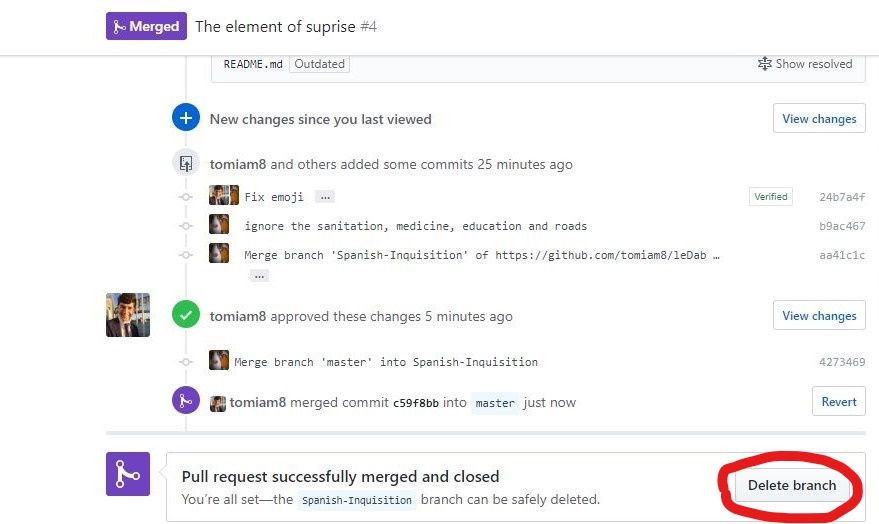
\includegraphics[width=\textwidth]{BPRW/11delete-branch}
		\caption{``Easily defeat Birnam forest with this one weird trick.''}
	\end{figure}
	\item Now delete the branch on your local with ``git branch --delete your-branch'' or in the GUI go ``Branch \textgreater Delete''
	\begin{figure}[H]
		\centering
		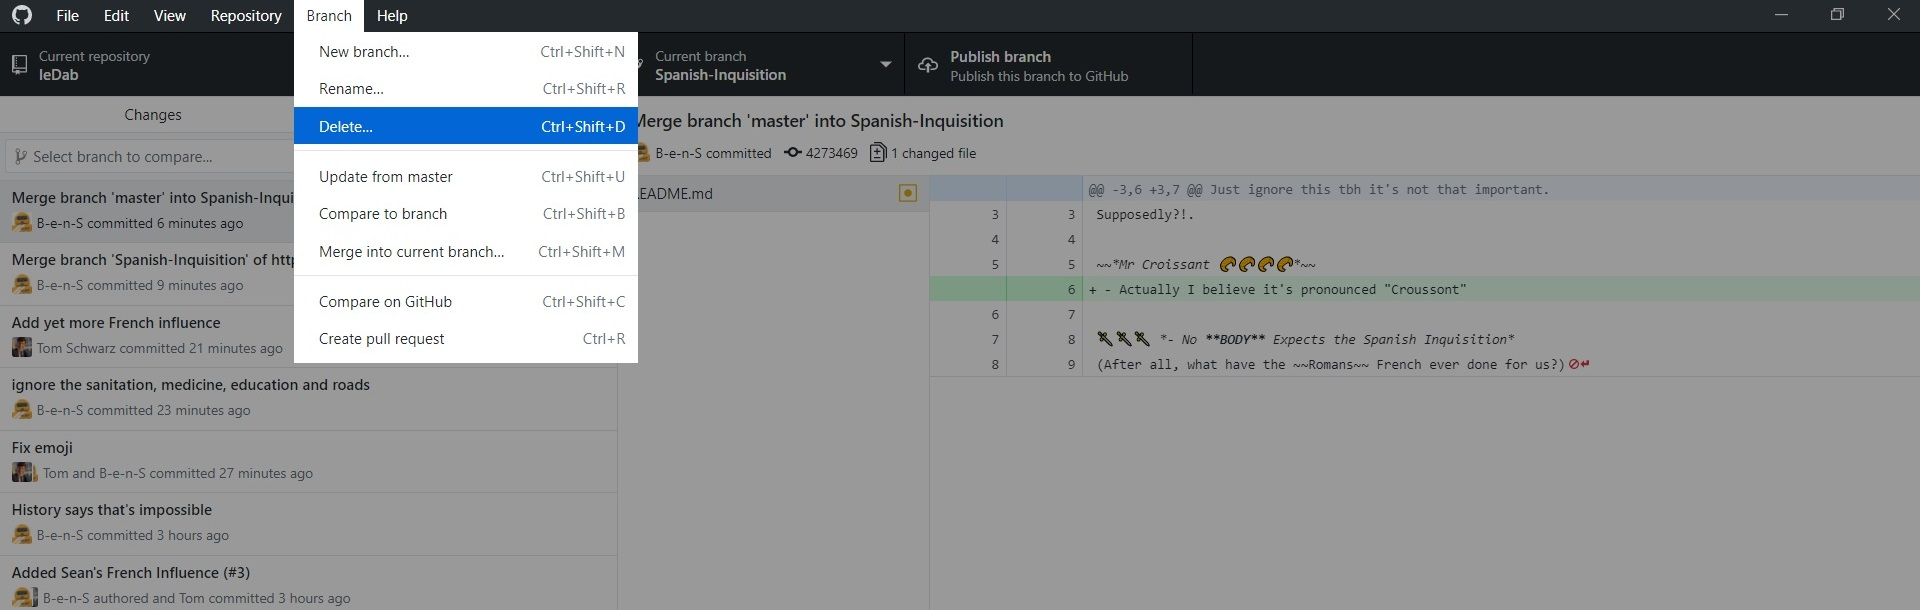
\includegraphics[width=\textwidth]{BPRW/12Delete-branch-github-desktop}
		\caption{``Don't tell Greenpeace.''}
	\end{figure}
\end{enumerate}
\begin{figure}[H]
	\centering
	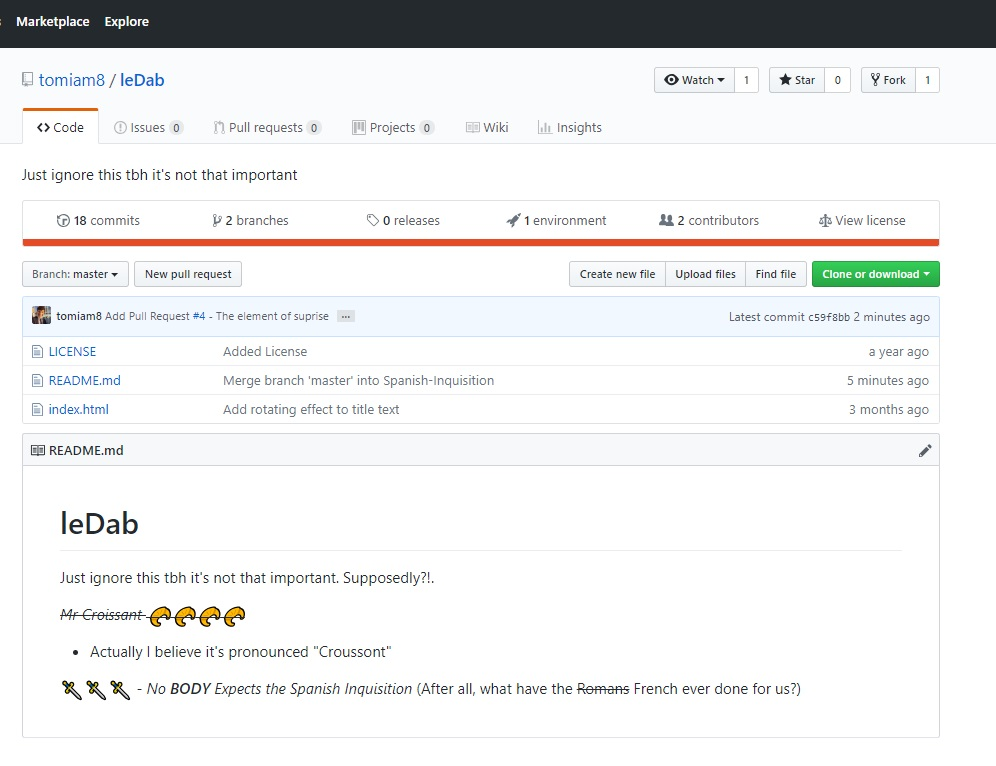
\includegraphics[width=\textwidth]{BPRW/13end-result}
	\caption{``Random monty python refrences counts as growing the (programming) python cult, right?''}
\end{figure}
	
\section{license}
This document (including the .tex, .pdf, included images and any other directly related files) uses the following modified MIT License:

Copyright (c) 2019 Thomas Schwarz
Copyright (c) 2019 relevant images authored by Ben Schwarz

Permission is hereby granted, free of charge, to any peron obtaining a copy of this document and any associated files (the ``document''), to deal in the document without restriction, including without limitation the rights to use, copy, modify, merge, publish, distribute, sublicense, and/or sell copies of the document, and to do so, subject to the following conditions:

The above copyright notice and this permission notice shall be included in all copies or substantial portions of the document.

THE DOCUMENT IS PROVIDED ``AS IS'', WITHOUT WARRANTY OF ANY KIND, EXPRESS OR IMPLIED, INCLUDING BUT NOT LIMITED TO THE WARRANTIES OF MERCHANTABILITY, FITNESS FOR A PARTICULAR PURPOSE AND NONINFRINGEMENT. IN NO EVENT SHALL THE AUTHORS OR COPYRIGHT HOLDERS BE LIABLE FOR ANY CLAIM, DAMAGES OR OTHER LIABILITY, WHETHER IN AN ACTION OF CONTRACT, TORT OR OTHERWISE, ARISING FROM, OUT OF OR IN CONNECTION WITH THE DOCUMENT OR THE USE OR DEALINGS IN THE DOCUMENT. THE USER ACCEPTS ALL RISK FROM USAGE OF THE DOCUMENT.

\end{document}